\documentclass{standalone}

\usepackage{tikz}
\usepackage{standalone}
\usetikzlibrary{calc}

\begin{document}
    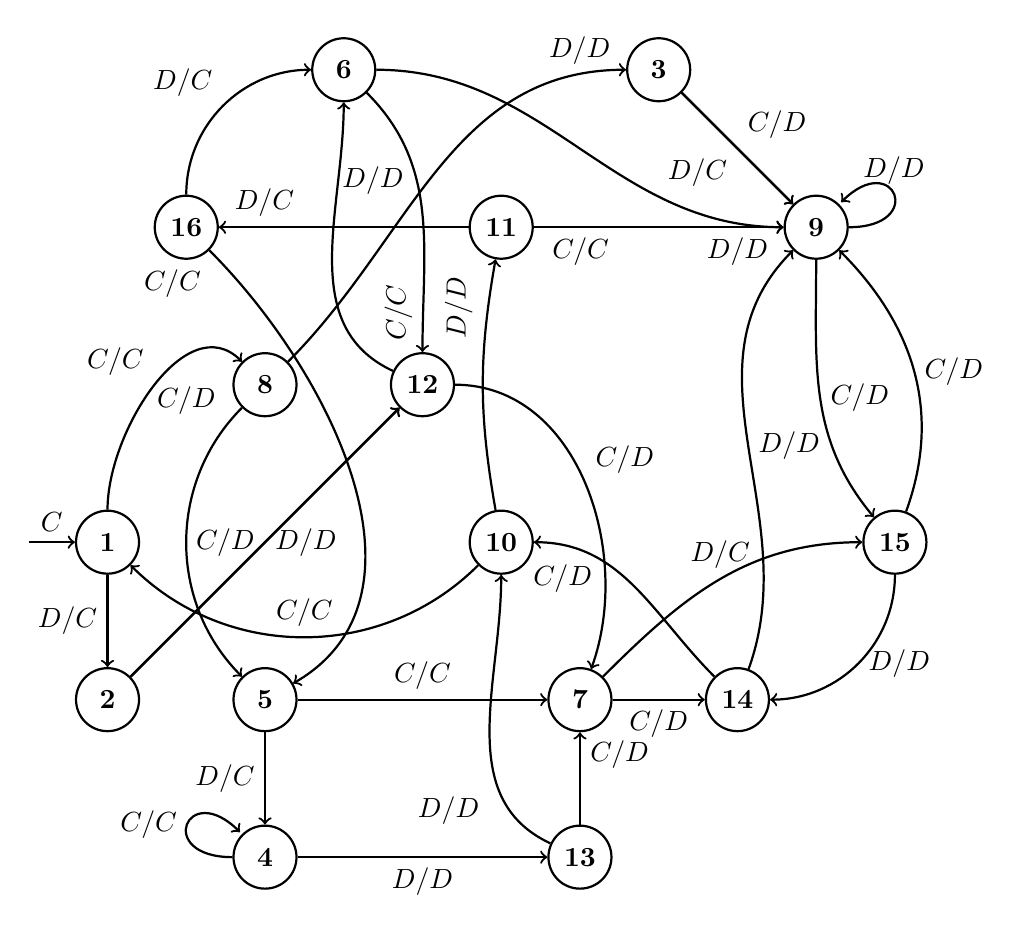
\begin{tikzpicture}

    \tikzstyle{state}=[minimum width=0.8cm, font=\boldmath];
    \node[circle, draw=black, thick] (5) at (0, 0) [state] {$6$};
	\node[circle, draw=black, thick] (2) at (4, 0) [state] {$3$};
	\node[circle, draw=black, thick] (15) at (-2, -2) [state] {$16$};
	\node[circle, draw=black, thick] (8) at ($(2)+(2,-2)$) [state] {$9$};
	\node[circle, draw=black, thick] (10) at ($(15)+(4, 0)$) [state] {$11$};
	
	\node[circle, draw=black, thick] (7) at ($(5)+(-1,-4)$) [state] {$8$};
	\node[circle, draw=black, thick] (11) at ($(7)+(2, 0)$) [state] {$12$};



	\node[circle, draw=black, thick] (9) at ($(10)+(0,-4)$) [state] {$10$};
	\node[circle, draw=black, thick] (0) at ($(9)+(-5,0)$) [state] {$1$};
	\node[circle, draw=black, thick] (14) at ($(9)+(5,0)$) [state] {$15$};

	\node[circle, draw=black, thick] (1) at ($(0)+(0,-2)$) [state] {$2$};
	\node[circle, draw=black, thick] (4) at ($(1)+(2,0)$) [state] {$5$};
	\node[circle, draw=black, thick] (6) at ($(4)+(4,0)$) [state] {$7$};
	\node[circle, draw=black, thick] (13) at ($(6)+(2,0)$) [state] {$14$};

	\node[circle, draw=black, thick] (3) at ($(4)+(0,-2)$) [state] {$4$};
	\node[circle, draw=black, thick] (12) at ($(6)+(0,-2)$) [state] {$13$};


    \coordinate[left of=0] (s);

    \draw (s) edge[out=0, in=180, ->, thick] node [above] {$C$} (0);
    \draw (0) edge[out=90, in=135, ->, thick] node [above left] {$C/C$} (7);
    \draw (0) edge[out=-90, in=90, ->, thick] node [left] {$D/C$} (1);

    \draw (1) edge[out=45, in=-135, ->, thick] node [left] {$C/D$} (11);
    \draw (1) edge[out=45, in=-135, ->, thick] node [right] {$D/D$} (11);
    
    \draw (2) edge[out=-45, in=135, ->, thick] node [above right] {$C/D$} (8);
    \draw (2) edge[out=-45, in=135, ->, thick] node [below left] {$D/C$} (8);

    \draw (3) edge[out=180, in=135, ->, thick, loop] node [left] {$C/C$} (3);
    \draw (3) edge[out=0, in=180, ->, thick] node [below] {$D/D$} (12);

    \draw (4) edge[out=0, in=180, ->, thick] node [above] {$C/C$} (6);
    \draw (4) edge[out=-90, in=90, ->, thick] node [left] {$D/C$} (3);

    \draw (5) edge[out=0, in=180, ->, thick] node [below, yshift=-1cm, xshift=2cm] {$D/D$} (8);
    \draw (5) edge[out=-45, in=90, ->, thick] node [left, yshift=-0.8cm, xshift=-0.3cm, rotate=90] {$C/C$} (11);

    \draw (6) edge[out=0, in=180, ->, thick] node [below] {$C/D$} (13);
    \draw (6) edge[out=45, in=180, ->, thick] node [above] {$D/C$} (14);

    \draw (7) edge[out=-135, in=135, ->, thick] node [yshift=1.8cm] {$C/D$} (4);
    \draw (7) edge[out=45, in=180, ->, thick] node [above, yshift=1.2cm, xshift=1.8cm] {$D/D$} (2);

    \draw (8) edge[out=0, in=45, ->, thick, loop] node [above] {$D/D$} (8);
    \draw (8) edge[out=-90, in=130, ->, thick] node [right] {$C/D$} (14);

    \draw (9) edge[out=-135, in=-45, ->, thick] node [above] {$C/C$} (0);
    \draw (9) edge[out=100, in=-100, ->, thick] node [above left, yshift=1.5cm, rotate=90] {$D/D$} (10);

    \draw (10) edge[out=0, in=180, ->, thick] node [below left, xshift=-0.5cm] {$C/C$} (8);
    \draw (10) edge[out=180, in=0, ->, thick] node [above left, xshift=-0.5cm] {$D/C$} (15);

    \draw (11) edge[out=0, in=70, ->, thick] node [above right] {$C/D$} (6);
    \draw (11) edge[out=155, in=-90, ->, thick] node [right, yshift=1cm] {$D/D$} (5);

    \draw (12) edge[out=90, in=-90, ->, thick] node [above right] {$C/D$} (6);
    \draw (12) edge[out=155, in=-90, ->, thick] node [left, yshift=-1cm] {$D/D$} (9);

    \draw (13) edge[out=135, in=0, ->, thick] node [below left, xshift=-0.4cm, yshift=0.4cm] {$C/D$} (9);
    \draw (13) edge[out=70, in=-135, ->, thick] node [right] {$D/D$} (8);

    \draw (14) edge[out=70, in=-45, ->, thick] node [right] {$C/D$} (8);
    \draw (14) edge[out=-90, in=0, ->, thick] node [right] {$D/D$} (13);

    \draw (15) edge[out=-45, in=30, ->, thick] node [left, xshift=-1.8cm, yshift=2.5cm] {$C/C$} (4);
    \draw (15) edge[out=90, in=180, ->, thick] node [above left] {$D/C$} (5);

    \end{tikzpicture}
\end{document}